% 图 C.1 玻尔模型：核电荷 Ze，电子 e- 在半径 r 的圆轨道上
\documentclass[tikz,border=5pt]{standalone}
\usetikzlibrary{arrows.meta}
\usepackage{amsmath}
\usepackage{bm}
\usepackage{fontspec}
\setmainfont{Times New Roman}
\begin{document}
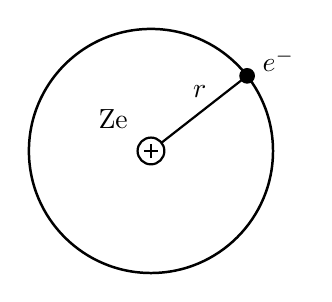
\begin{tikzpicture}[line width=0.8pt,>=Stealth]
% orbit
\draw[line width=0.9pt] (0,0) circle (1.55);
% nucleus
\draw[line width=0.8pt,fill=white] (0,0) circle (0.17);
\draw[line width=0.8pt] (-0.09,0) -- (0.09,0);
\draw[line width=0.8pt] (0,-0.09) -- (0,0.09);
\node at (-0.48,0.40) {Ze};
% radius and electron
\draw[line width=0.8pt] (0.134,0.105) -- (1.221,0.954);
\node[above] at (0.62,0.55) {$r$};
\fill (1.221,0.954) circle (0.10);
\node at (1.62,1.15) {$e^-$};
\end{tikzpicture}
\end{document}
